\documentclass{article}

\usepackage{fullpage}
\usepackage{amsmath}
\usepackage{amsfonts}
\usepackage{bm}
\usepackage{graphicx}

\newcommand{\dx}{{\Delta x}}
\newcommand{\dV}{{\Delta V}}
\newcommand{\dt}{{\Delta t}}
\newcommand{\Nc}{{N_\mathrm{c}}}
\newcommand{\nb}{\bar{n}}
\newcommand{\Nav}{{N_\mathrm{av}}}

\begin{document}

\title{The Equilibrium Distribution of Cell Number Density}
\author{}
\date{}
\maketitle

\section{\label{sec_overview}Overview}

In this report, we obtain the analytic expression for the equilibrium distribution~$\rho(n)$ of cell number density~$n$ in the one-dimensional diffusion system subject to stochastic flux.
In addition, we discuss how the resulting \textit{continuous} distribution and the physically-correct \textit{discrete} distribution based on the Poisson statistics can match each other as the average number of particles per cell increases. 
Combined with the previous analysis on the second-order statistics, this analysis provides full understanding on the equilibrium distribution of the system.
\\

\noindent Analyzing the continuous-time spatially-discretized system (see below a set of SODEs given in Eq.~\eqref{sode}) is important, since numerical schemes are based on this system rather than the original SPDE (see below Eq.~\eqref{spde}).
One thing to note is that the connection between the SPDE and the SODEs are not so rigorous but rather heuristic.
In fact, there is no convergence theorem for the limit $\dx\rightarrow0$.
This limit is also physically strange in the sense that the number of particles in a cell eventually becomes zero.
Moreover, as it is, the SPDE is mathematically ill-defined due to the occurrence of negative densities.
On the other hand, we will see that there is more room for handling negative densities in the SODEs so that they can be well-defined and attain the equilibrium state.
In addition, the concept of cell number density, which is introduced when the SPDEs are heuristically obtained from the SPDE by the idea of the finite volume method, has a perfect physical meaning and enables a direct comparison with the physical system.
However, until now, little has been analytically known about how the SODEs system can mimic the physical system.
For example, it is a non-trivial quation how the continous distribution generated by the SODEs can agree with the physically-correct discrete distribution based on the Poisson statistics.
Lastly, by considering the fact that a numerical scheme converges to the SODEs in the limit $\dt\rightarrow0$, analytic expressions for equilibrium properties such as the structure factor and the cell number density distribution are helpful to understand the scheme. 
\\

\noindent In Section~\ref{sec_sodes}, we introduce the governing SODEs and discuss some issues related to the well-definedness.
In Section~\ref{sec_main_res}, we summarize the main results of this report.
In Section~\ref{sec_deriv_de_rho1}, we derive a differential equation of $\rho(n)$, from which the main results are obtained.
In Section~\ref{sec_discuss}, we discuss the validity of our results.

\section{\label{sec_sodes}Governing SODEs}

The one-dimensional diffusion equation subject to stochastic flux is written as follows: 
\begin{equation}
\label{spde}
\frac{\partial}{\partial t}n(x,t)
=\chi\frac{\partial^2}{\partial x^2}n(x,t)
+\frac{\partial}{\partial x}\left[
\sqrt{\frac{2\chi n(x,t)}{A}}\bm{\mathcal{W}}(x,t)
\right],
\end{equation}
where $n(x,t)$ and $\bm{\mathcal{W}}(x,t)$ are the number density and a spatio-temporal Gaussian white noise process, respectively, and $\chi$ and $A$ are the diffusion coefficient and the cross section area of the system, respectively.
Since $n(x,t)$ is driven by $\bm{\mathcal{W}}(x,t)$, the value of $n(x,t)$ at a certain position $x$ may not be so meaningful.
In other words, even if a solution of Eq.~\eqref{spde} exists, it may not be continuous with respect to $x$.
Hence, borrowing the idea of the finite volume method, the domain is divided into a grid of cells of size $\dx$ and the following set of SODEs for cell number densities $n_j$ is obtained:
\begin{equation}
\label{sode}
\frac{d}{dt}n_j(t)=\chi\frac{n_{j+1}(t)+n_{j-1}(t)-2n_j(t)}{\dx^2}
+\frac{1}{\dx}\left(
\sqrt{\frac{2\chi\tilde{n}_{j+\frac12}(t)}{\dV}}W_{j+\frac12}(t)
-\sqrt{\frac{2\chi\tilde{n}_{j-\frac12}(t)}{\dV}}W_{j-\frac12}(t)
\right).
\end{equation}
Here, the deterministic diffusion part is expressed by the discrete Laplacian, whereas the stochastic diffusive flux between cells $j$ and $j+1$ is expressed in terms of the face value $\tilde{n}_{j+\frac12}$ and an independent Gaussian white noise process $W_{j+\frac12}$.
Note that the cross section $A$ in Eq.~\eqref{spde} has been replaced by the cell volume $\dV=A\dx$ due to the spatial integration.
To close Eq.~\eqref{sode}, $\tilde{n}_{j+\frac12}$ is expressed as a function of $n_j$ and $n_{j+1}$:
\begin{equation}
\tilde{n}_{j+\frac12}=\tilde{n}(n_j,n_{j+1}).
\end{equation}
Since the face value $\tilde{n}$ should be close to the two center values, natural candidates for $\tilde{n}$ would be averages of these two values such as the Pythagorean means.

In order for Eq.~\eqref{sode} to attain a mathematically well-defined solution, the following criteria on $\tilde{n}$ should be taken into consideration.
First of all, it should be non-negative.
This obvious criterion may not hold if Eq.~\eqref{sode} happens to allow negative densities.
For the arithmetic mean (AM),
\begin{equation}
\tilde{n}^\mathrm{AM}(n_1,n_2)=\frac12(n_1+n_2),
\end{equation}
its value can be negative if $n_1$ or $n_2$ becomes negative.
Secondly, $\tilde{n}(n_1,n_2)$ should be well-defined even if $n_1$ or $n_2$ is negative.
Note that the geometric mean (GM) and the harmonic mean (HM) are not well-defined in this case.
One possible remedy for these issues is to set the value of $\tilde{n}$ zero if $n_1$ or $n_2$ is negative.
That is, for the AM, the remedy suggests
\begin{equation}
\label{tildenAMP}
\tilde{n}^\mathrm{AM,+}(n_1,n_2)=\frac12(n_1+n_2)H(n_1)H(n_2),
\end{equation}
where $H$ is the Heaviside step function.
Note that Eq.~\eqref{sode} becomes robust with this remedy in the sense that even if negative densities occur, each term in Eq.~\eqref{sode} is well-defined.
Also, if a cell happens to have a negative density, all stochastic fluxes through its faces are turned off.
Note that this prevents the cell number density from becoming more negative.

In this report, we analyze the equilibrium cell number density distribution of Eq.~\eqref{sode} with $\tilde{n}$ satisfying
\begin{equation}
\label{cond}
\tilde{n}(n_1,n_2) = 0\quad\mbox{if $n_1<0$ or $n_2<0$}.
\end{equation}
We also assume that there are $\Nc$ cells under prediodic boundary condition.
In Eq.~\eqref{sode}, the sum of cell number densities is strictly conserved:
\begin{equation}
\sum_{j=1}^\Nc n_j(t)=\Nc\nb.
\end{equation}
Here, we have introduce the equilibrium number density $\nb$.

\section{\label{sec_main_res}Main Results}

The main results of this report are two-fold.
In Section~\ref{subsec_main_res_gen}, we summarize the results for a \textit{general} $\tilde{n}$.
We derive a differential equation for $\rho(n)$ and then obtain its solution.
In Section~\ref{subsec_main_res_AMNav}, we present \textit{closed-form} expressions for $\tilde{n}^{\mathrm{AM},+}$ in the regime $\nb\dV\gg 1$ (i.e., having a large number of particles per cell), and then compare them with the Poisson statistics.

\subsection{\label{subsec_main_res_gen}General Case}

\paragraph{Differential Equation for $\bm{\rho_1(n_1)}$}

Because of no preference among cells due to periodic boundary condition, it suffices to investigate the equilibrium distribution of the cell number density of cell 1, which is denoted by $\rho_1(n_1)$.
In other words, we need to calculate the marginial distribution $\rho_1(n_1)$ from the equilibrium distribution $\rho_\mathrm{eq}(n_1,n_2,\dots,n_\Nc)$.
In Section~\ref{sec_deriv_de_rho1}, by integrating the Fokker--Planck equation of $\rho(n_1,n_2,\dots,n_\Nc,t)$, we obtain the following differential equation of $\rho_1(n_1)$:
\begin{equation}
\label{de_rho1}
\dV\left[\langle n_2|n_1\rangle-n_1\right]\rho_1(n_1)=\frac{d}{d n_1}\left[\langle\tilde{n}(n_1,n_2)|n_1\rangle\rho_1(n_1)\right],
\end{equation}
where $\langle n_2|n_1\rangle$ is the conditional expectation of the cell number density of adjacent cell (i.e., $n_2$) given $n_1$ and $\langle\tilde{n}(n_1,n_2)|n_1\rangle$ is that of the face value $\tilde{n}(n_1,n_2)$.
Note that these two conditional expectations are functions of $n_1$ and, in principle, can be calculated from the marginal distribution $\rho_{1,2}(n_1,n_2)$.

\paragraph{Expression of $\bm{\rho_1(n_1)}$ (general case)}

Since Eq.~\eqref{de_rho1} is a first-order ODE, it can be readily solved and expressed in terms of $\langle n_2|n_1\rangle$ and $\langle\tilde{n}(n_1,n_2)|n_1\rangle$ as follows:
\begin{equation}
\label{expr_rho1_gen}
\rho_1(n_1)=\frac{C(n^*)}{\langle\tilde{n}(n_1,n_2)|n_1\rangle}\exp\left[\dV\int_{n^*}^{n_1} \frac{\langle n_2|n_1'\rangle-n_1'}{\langle\tilde{n}(n_1',n_2)|n_1'\rangle}dn_1'\right],
\end{equation}
where $n^*$ can be any number belonging to the maximal interval of existence of the solution $\rho_1(n_1)$ and $C(n^*)$ can be determined by the normalization condition $\int \rho_1(n_1)dn_1=1$.

\subsection{\label{subsec_main_res_AMNav}$\bm{\tilde{n}^{\mathrm{AM},+}}$ and $\bm{\nb\dV\gg 1}$}

\paragraph{Expressions of $\bm{\langle n_2|n_1\rangle}$ and $\bm{\langle\tilde{n}|n_1\rangle}$}

In order to derive a closed-form expression from Eq.~\eqref{expr_rho1_gen}, we need closed-form of $\langle n_2|n_1\rangle$ and $\langle\tilde{n}(n_1,n_2)|n_1\rangle$.
From the conservation of total sum of cell number densities, the following expression of $\langle n_2|n_1\rangle$ is proposed:
\begin{equation}
\label{expr_n2n1}
\langle n_2|n_1\rangle = \frac{\Nc\nb-n_1}{\Nc-1}.
\end{equation}
If fact, Eq.~\eqref{expr_n2n1} can be obtained by assuming that $\langle n_j|n_1\rangle$ $(j\ne1)$ does not depend on $j$.
In Appendix~A, it is numerically verified that this assumption and Eq.~\eqref{expr_n2n1} hold.
On the other hand, as the average number of particles per cell, denoted by $\Nav$, becomes larger, the cell number density becomes more narrowly distributed around $\nb$.
In this case, even if the equilibrium distribuion possibly allows negative densities, the probability of negative density becomes asymptotically zero.
Hence, for $\tilde{n}^{\mathrm{AM},+}$, we may assume that 
\begin{equation}
\label{expr_ntilden1}
\langle\tilde{n}^{\mathrm{AM},+}(n_1,n_2)|n_1\rangle\approx
\frac12\left(n_1+\langle n_2|n_1\rangle\right).
\end{equation}

\paragraph{Asymptotic expression of $\bm{\rho_1(n_1)}$}

By substituting Eqs.~\eqref{expr_n2n1} and \eqref{expr_ntilden1} into Eq.~\eqref{expr_rho1_gen}, we obtain
\begin{equation}
\label{expr_rho1_AMNav}
\rho_1(n_1)=C\exp\left[-2\left(\frac{1-\zeta}{1+\zeta}\right)n_1\dV\right]\left[1+\frac{1+\zeta}{1-\zeta}\frac{n_1}{\nb}\right]^{\frac{4\nb\dV}{1+\zeta}-1}
\end{equation}
where
\begin{equation}
\zeta = -\frac{1}{\Nc-1},
\end{equation}
and $C$ is determined from the normalization condition.
Since $\zeta\rightarrow 0$ as $\Nc\rightarrow\infty$, in the infinite system, $\rho_1(n_1)$ becomes
\begin{equation}
\label{expr_rho1_AMNav_inf}
\rho_1(n_1) = C(\nb,\dV)e^{-2n_1\dV}\left(1+\frac{n_1}{\nb}\right)^{4\nb\dV-1}.
\end{equation}
Here, from $\int_0^\infty\rho_1(n_1)dn_1=1$, $C(\nb,\dV)$ is expressed as
\begin{equation}
C(\nb,\dV)=\frac{1}{\nb e^{2\nb\dV} E_{1-4\nb\dV}(2\nb\dV)},
\end{equation}
where $E_\nu(z)$ is the exponential integral function.

\paragraph{Comparison with the Poisson statistics}

From Eq.~\eqref{expr_rho1_AMNav_inf}, we also obtain the expression for the distribution $\rho_N(N)$ of the number of particles in a cell $N$ as follows:
\begin{equation}
\label{rhoN}
\rho_N(N)=C(\Nav)e^{-2N}\left(1+\frac{N}{\Nav}\right)^{4\Nav-1}.
\end{equation}
Here, from $\int_0^\infty \rho_N(N)dN=1$, we have
\begin{equation}
C(\Nav)=\frac{1}{\Nav e^{2\Nav}E_{1-4\Nav}(2\Nav)}.
\end{equation}

If $\rho_N(N)$ is a physically right answer, it is expected that, as $\Nav$ becomes larger, $\rho_N(N)$ becomes more similar to the Poisson distribution $P(N)$ with mean $\Nav$:
\begin{equation}
\label{Poisson}
P(N)=\frac{e^{-\Nav}\Nav^N}{N!},\quad\mbox{for $N=0,1,2,\dots$}.
\end{equation}
By noting that the gamma function $\Gamma(x)$ satisfies $\Gamma(k+1)=k!$ for non-negative integer $k$, we have the following continuous distribution, which approximates to $P(N)$: 
\begin{equation}
\label{Papprox1}
\rho^\mathrm{Poisson}_\mathrm{approx,1}(N)=C_1(\Nav)\frac{e^{-\Nav}\Nav^N}{\Gamma(N+1)}.
\end{equation}
By applying Stirling's approximation to $N!$ and then the continuity correction, we also obtain
\begin{equation}
\label{Papprox2}
\rho^\mathrm{Poisson}_\mathrm{approx,2}(N)=C_2(\Nav)e^{N+\frac12}\left(\frac{\Nav}{N+\frac12}\right)^{N+\frac12}.
\end{equation}

\begin{figure}
\begin{center}
\begin{tabular}{cc}
$\Nav=10$ & $\Nav=50$ \\
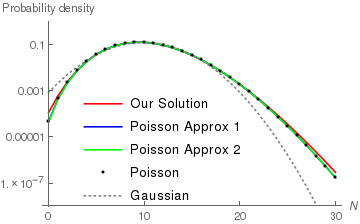
\includegraphics[width=0.4\linewidth]{fig4/rho_Nav10.png} &
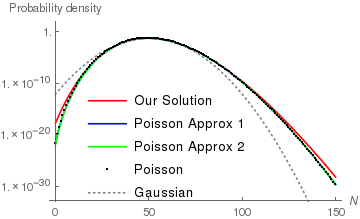
\includegraphics[width=0.4\linewidth]{fig4/rho_Nav50.png}
\end{tabular}
\caption{\label{fig_rho}Continuous distribution of $\rho_N(N)$ (our solution, Eq.~\eqref{rhoN}), $\rho^\mathrm{Poisson}_\mathrm{approx,1}(N)$ (Eq.~\eqref{Papprox1}), and $\rho^\mathrm{Poisson}_\mathrm{approx,2}(N)$ (Eq.~\eqref{Papprox2}) are compared with the Poisson distribution $P(N)$ (Eq.~\eqref{Poisson}) for $\Nav=10$ (in the left panel) and 50 (in the right panel). The Gaussian distribution with mean $\Nav$ and variance $\Nav$ is also plotted.}
\end{center}
\end{figure}
\begin{figure}
\begin{center}
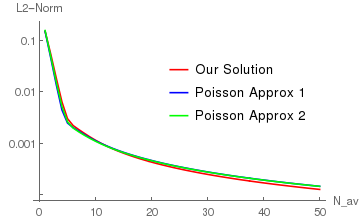
\includegraphics[width=0.4\linewidth]{fig4/L2norm.png}
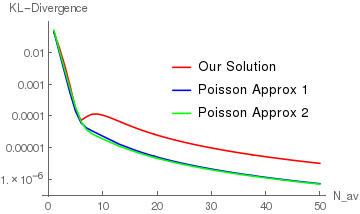
\includegraphics[width=0.4\linewidth]{fig4/KLdiv.png}
\caption{\label{fig_L2norm_KLdiv}In the left pannel, the $L^2$-differences of $\rho_N(N)$, $\rho^\mathrm{Poisson}_\mathrm{approx,1}(N)$, and $\rho^\mathrm{Poisson}_\mathrm{approx,2}(N)$ from the Poisson distribution $P(N)$ are plotted versus $\Nav$. In the right pannel, the KL-divergences of these distributions with respect to $P(N)$ are plotted versus $\Nav$. For the definitions of the $L^2$-difference and the KL-divergence, see Eqs.~\eqref{L2norm} and \eqref{KLdiv}.}
\end{center}
\end{figure}
\begin{figure}[t!]
\begin{center}
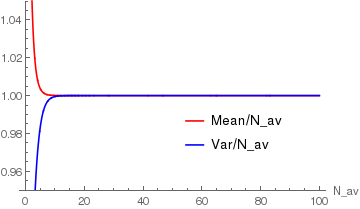
\includegraphics[width=0.4\linewidth]{fig4/meanvar.png}
\caption{\label{fig_meanvar}The mean and variance of our solution $\rho_N(N)$ are plotted versus $\Nav$.}
\end{center}
\end{figure}
In Fig.~\ref{fig_rho}, we compare continuous distributions $\rho_N(N)$, $\rho^\mathrm{Poisson}_\mathrm{approx,1}(N)$ and $\rho^\mathrm{Poisson}_\mathrm{approx,2}(N)$ with the Poisson distribution $P(N)$ for $\Nav=10$ and 50.
Our solution $\rho_N(N)$ is very similar to the Poisson distribution in a large range, but the decay of the tails of $\rho_N(N)$ is slightly slower than the Poisson distribution. 
In Fig.~\ref{fig_L2norm_KLdiv}, we also calculate the deviations of each continuous distribution from $P(N)$ for the following measures.
The first one is the $L^2$-norm of a continuos distribuion $f$ and $P(N)$ defined as  
\begin{equation}
\label{L2norm}
d_{L^2}(f)=\sum_{k=0}^\infty \left(P(k)-\int_{(k-\frac12)^+}^{k+\frac12}f(N)dN\right)^2.
\end{equation}
Note that the plus superscript is used for the lower limit of the integral for $k=0$.
The other one is the Kullback-Leibler (KL) divergence of $f$ with respect to $P(N)$ defined as
\begin{equation}
\label{KLdiv}
d_{KL}(f)=\sum_{k=0}^\infty P(k)\log\left(\frac{P(k)}{\int_{(k-\frac12)^+}^{k+\frac12}f(N)dN}\right).
\end{equation}
Finally, in Fig.~\ref{fig_meanvar}, we show that the mean $\bar{N}$ and variance $\mathrm{Var}[N]$ of $\rho_N(N)$ becomes $\Nav$ if $\Nav$ is sufficiently large.
In fact, it can be analytically shown that 
\begin{equation}
\lim_{\Nav\rightarrow\infty}\frac{\bar{N}}{\Nav}=1,\quad \lim_{\Nav\rightarrow\infty}\frac{\mathrm{Var}[N]}{\Nav}=1.
\end{equation}

\section{\label{sec_deriv_de_rho1}Derivation: Differential Equation~\eqref{de_rho1} of $\bm{\rho_1(n_1)}$}

A vector-form equation of Eq.~\eqref{sode} is written as
\begin{equation}
\frac{d}{dt}\mathbf{n}(t)=\frac{\chi}{\Delta x^2}D\mathbf{n}(t)+\frac{\sqrt{2\chi}}{\dx\sqrt{\dV}}F(\mathbf{n}(t))\mathbf{W}(t).
\end{equation}
where, for example, for $\Nc=4$, $\mathbf{n}(t)=\left[n_1(t),n_2(t),n_3(t),n_4(t)\right]$, $\mathbf{W}(t)=\left[W_{1,2}(t),W_{2,3}(t),W_{3,4}(t),W_{4,1}(t)\right]$,
\begin{equation}
D=\left[
\begin{array}{cccc}
-2 & 1 & 0 & 1 \\
1 & -2 & 1 & 0 \\
0 & 1 & -2 & 1 \\
1 & 0 & 1 & -2
\end{array}
\right],
\end{equation}
\begin{equation}
F(\mathbf{n})=\left[
\begin{array}{cccc}
\sqrt{\tilde{n}(n_1,n_2)} & 0 & 0 & -\sqrt{\tilde{n}(n_4,n_1)} \\
-\sqrt{\tilde{n}(n_1,n_2)} & \sqrt{\tilde{n}(n_2,n_3)} & 0 & 0 \\
0 & -\sqrt{\tilde{n}(n_2,n_3)} & \sqrt{\tilde{n}(n_3,n_4)} & 0 \\
0 & 0 & -\sqrt{\tilde{n}(n_3,n_4)} & \sqrt{\tilde{n}(n_4,n_1)} \\
\end{array}
\right].
\end{equation}
The Fokker-Planck equation of the probability density $\rho(\mathbf{n},t)=\rho(n_1,n_2,\dots,n_\Nc,t)$ is written as
\begin{equation}
\frac{\partial}{\partial t}\rho(\mathbf{n},t)
=-\frac{\chi}{\dx^2}\sum_{j=1}^\Nc \frac{\partial}{\partial n_j}\left[(D\mathbf{n})_j\rho\right]
+\frac{\chi}{\dx^2\dV}\sum_{j=1}^\Nc\sum_{j'=1}^\Nc \frac{\partial^2}{\partial n_j\partial n_j'}\left[\left(F(\mathbf{n})F^T(\mathbf{n})\right)_{j,j'}\rho\right].
\end{equation}
The equilibrium distribution $\rho_\mathrm{eq}(\mathbf{n})$ satisfies
\begin{equation}
\label{FKE_eq}
-\frac{\chi}{\dx^2}\sum_{j=1}^\Nc \frac{\partial}{\partial n_j}\left[(D\mathbf{n})_j\rho_\mathrm{eq}(\mathbf{n})\right]
+\frac{\chi}{\dx^2\dV}\sum_{j=1}^\Nc\sum_{j'=1}^\Nc \frac{\partial^2}{\partial n_j\partial n_j'}\left[\left(F(\mathbf{n})F^T(\mathbf{n})\right)_{j,j'}\rho_\mathrm{eq}(\mathbf{n})\right]=0.
\end{equation}
Before integrating Eq.~\eqref{FKE_eq} with respect to $n_2,\dots,n_\Nc$, we define the marginal pdf of $n_1$ and the conditional pdf given $n_1$ as follows:
\begin{align}
&\rho_1(n_1)=\int d n_2 \dots d n_\Nc \rho_\mathrm{eq}(n_1,n_2,\dots,n_\Nc),\\
&\rho_{n_1}(n_2,\dots,n_\Nc)= \frac{\rho_\mathrm{eq}(n_1,n_2,\dots,n_\Nc)}{\rho_1(n_1)}.
\end{align}
By assuming that the boundary values are zero\footnote{This is not trivial. See Section~\ref{subsec_maxintv}.}, all terms containing a partial derivative with respect to $n_j$ with $j\ne1$ disappear after integrating Eq.~\eqref{FKE_eq} with respect to $n_j$ with $j\ne1$.
Then, by using
\begin{equation}
\begin{split}
&\int d n_2 \dots d n_\Nc\; f(n_1,n_2,\dots,n_\Nc)\rho_\mathrm{eq}(n_1,n_2,\dots,n_\Nc)\\
&=\rho_1(n_1)\int d n_2\dots d n_\Nc\; f(n_1,n_2,\dots,n_\Nc)\rho_{n_1}(n_2,\dots,n_\Nc)\\
&=\rho_1(n_1)\langle f(n_1,n_2,\dots,n_\Nc)|n_1\rangle
\end{split}
\end{equation}
and
\begin{equation}
(D\mathbf{n})_1 = n_2+n_\Nc-2n_1,\quad \left(F(\mathbf{n})F^T(\mathbf{n})\right)_{1,1}=\tilde{n}(n_1,n_2)+\tilde{n}(n_1,n_\Nc),
\end{equation}
we obtain 
\begin{equation}
-\frac{\partial}{\partial n_1}\left[\left(\langle n_2|n_1\rangle+\langle n_\Nc|n_1\rangle-2n_1\right)\rho_1(n_1)\right]
+\frac{1}{\dV}\frac{\partial^2}{\partial n_1^2}\left[\left(\langle\tilde{n}(n_1,n_2)|n_1\rangle+\langle\tilde{n}(n_1,n_\Nc)|n_1\rangle\right)\rho_1(n_1)\right]=0.
\end{equation}
Since $\langle n_2|n_1\rangle=\langle n_\Nc|n_1\rangle$ and $\langle\tilde{n}(n_1,n_2)\rangle=\langle\tilde{n}(n_1,n_\Nc)\rangle$, we finally obtain Eq.~\eqref{de_rho1}.

\section{\label{sec_discuss}Discussion}

\subsection{\label{subsec_maxintv}Maximal Interval of Existence and Condition for Non-Negative Densities}

The form of the solution $\rho_1(n_1)$ in the general case, given in Eq.~\eqref{expr_rho1_gen}, suggests that the maximal interval of existence of $\rho_1(n_1)$ cannot extend beyond a point satisfying $\langle\tilde{n}(n_1,n_2)|n_1\rangle=0$.
From the condition given in Eq.~\eqref{cond}, we have $\langle\tilde{n}(n_1,n_2)|n_1\rangle=0$ for $n_1<0$.
Then, this implies that $\rho_1(n_1)$ cannot be defined for $n_1<0$ and for the maximal interval of existence, denoted by $(n_\mathrm{min},\infty)$, we have $n_\mathrm{min}\ge0$.
This seems favorable in the sense that condition~\eqref{cond} gurantees non-negative densities of the equilibrium distribution.
However, under this type of the maximal interval of existence, the derivation of differential equation~\eqref{de_rho1} for $\rho_1(n_1)$ needs an additional assumption that the equilibrium distribution $\rho_\mathrm{eq}(n_1,n_2,\dots,n_\Nc)$ smoothly becomes zero as $n_j\rightarrow n_\mathrm{min}$ ($j=1,\dots,\Nc$).
This is needed to ignore boundary value terms when $\rho_\mathrm{eq}(n_1,n_2,\dots,n_\Nc)$ is integrated with respect to $n_2,\dots,n_\Nc$.
To this end, an additional condition such as a regularity condition for $\tilde{n}$ like $\tilde{n}(n_1,n_2)$ should be smooth at $n_1=0$ or $n_2=0$ is expected to be required in order that our results in the general case \textit{exactly} hold.
In this case, a possible scinario is that $n_\mathrm{min}=0$, $\lim_{n\rightarrow 0^+}\rho(n)=0$, and the Poisson distribution value $P(0)$ at $N=0$ can be compared with the value $\int_0^{\frac{1}{2}}\rho_N(N)dN$.

\subsection{Validity of the Results for $\bm{\tilde{n}^\mathrm{AM,+}}$}

Since the sum of cell number densities is strictly conserved in Eq.~\eqref{sode}, the mean $\bar{N}$ of $\rho_N(N)$ should be $\Nav=\nb\dV$.
As shown in Fig.~\ref{fig_meanvar}, however, $\bar{N}$ is not equal to $\Nav$ for small values of $\Nav$.
This indicates that the assumption given in Eq.~\eqref{expr_ntilden1} does not hold in this case.
Hence, as mentioned, the analytic expression of $\rho(n)$ becomes asymptotically valid for $\nb\dV\gg 1$.

We can go around the regularity issue raised in Section~\ref{subsec_maxintv} by introduing a \textit{smoothed} Heaviside step function in Eq.~\eqref{tildenAMP}.
This modification will cause some change in the value of $\rho(n)$ at smaller values $n$ through $\langle\tilde{n}|n\rangle$, but it is expected from the form of solution\footnote{Choose $n^*=\nb$ in Eq.~\eqref{expr_rho1_gen}} (see Eq.~\eqref{expr_rho1_gen}) that the change is rather small and local around the region of very small values of $N$.

It is not clear whether the slight deviation from the Poisson distribution observed in the \textit{left}-hand side tail (i.e., smaller values of $N$) of $\rho_N(N)$ (see Fig.~\ref{fig_rho}) is due to the failure of the assumption for $\tilde{n}$ given in Eq.~\eqref{expr_ntilden1} or whether it is inherent in Eq.~\eqref{sode}.
However, it seems quite sure that the deviation observed in the \textit{right}-hand side tail (i.e., larger values of $N$) is not related to the failure of the assumption given in Eq.~\eqref{expr_ntilden1}.
Although slight deviations are observed in the tails from the Poisson distribution, $\rho_N(N)$ is much closer to the Poisson distribution and than to the Gaussian distribution.

\clearpage

\section*{Appendices}

\subsection*{A. Numerical Verification of Expression~\eqref{expr_n2n1} for $\langle n_2|n_1\rangle$}

\begin{figure}
\begin{center}
\includegraphics[angle=270,width=0.4\linewidth]{fig4/n1n2_Nc1024.eps}
\caption{\label{fig_condexp}For the system having $\Nc=1024$ cells with $\nb=1$ and $\dV=1000$, the values of $\langle n_2|n_1\rangle$ are plotted as functions of $n_1$ for $\Delta t = 0.01$, 0.02, 0.05, and 0.1 and compared with Eq.~\eqref{expr_n2n1}.}
\end{center}
\end{figure}

The expression of $\langle n_2|n_1\rangle$ given in Eq.~\eqref{expr_n2n1} is numerically confirmed by simulating Eq.~\eqref{sode} using a temporal integrator with small time steps.
More specifically, the system having $\chi=1$, $\nb=1$, $\dx=1$, and $A=1000$ was simulated by the implicit midpoint predictor-corrector scheme with $\dt=0.01$, 0.02, 0.05, and 0.1.
In order to minimize the finite-system-size effect, $\Nc=1024$ was chosen.
As shown in Fig.~\ref{fig_condexp}, for smaller time steps, numerical results agree very well with Eq.~\eqref{expr_n2n1}.
Note that for the regions with $n_1\gg\nb$ or $n_1\ll\nb$ the standard errors become larger because of small number of samples for averaging.

\subsection*{B. Numerical Results: Probability of Negative Cell Number Density}

\begin{figure}
\begin{center}
\includegraphics[angle=270,width=0.4\linewidth]{fig4/neg_dens.eps}
\caption{\label{fig_negdens}For the system having $\Nc=1024$ cells with $\nb=1$ and $\dV=10$, the probability of having negative cell number density is plotted as functions of $\Delta t$.}
\end{center}
\end{figure}

In order to numerically confirm that Eq.~\eqref{sode} does not allow negative cell number density, a diffusion-only system with $\Nc=1024$ was simulated by using a temporal integrator with small time steps $\Delta t=0.005$, 0.01, 0.02, 0.05, and 0.1.
As shown in Fig.~\ref{fig_negdens}, the probability of having negative cell number density quickly decreases to zero as $\Delta t\rightarrow 0$.

\end{document}
